% figures.tex — auto-generated by make_figures.py
% % figures.tex � auto-generated by make_figures.py
% % figures.tex � auto-generated by make_figures.py
% % figures.tex � auto-generated by make_figures.py
% \input{figures_output/figures.tex} in your main .tex file

\begin{figure}[htbp]
  \centering
  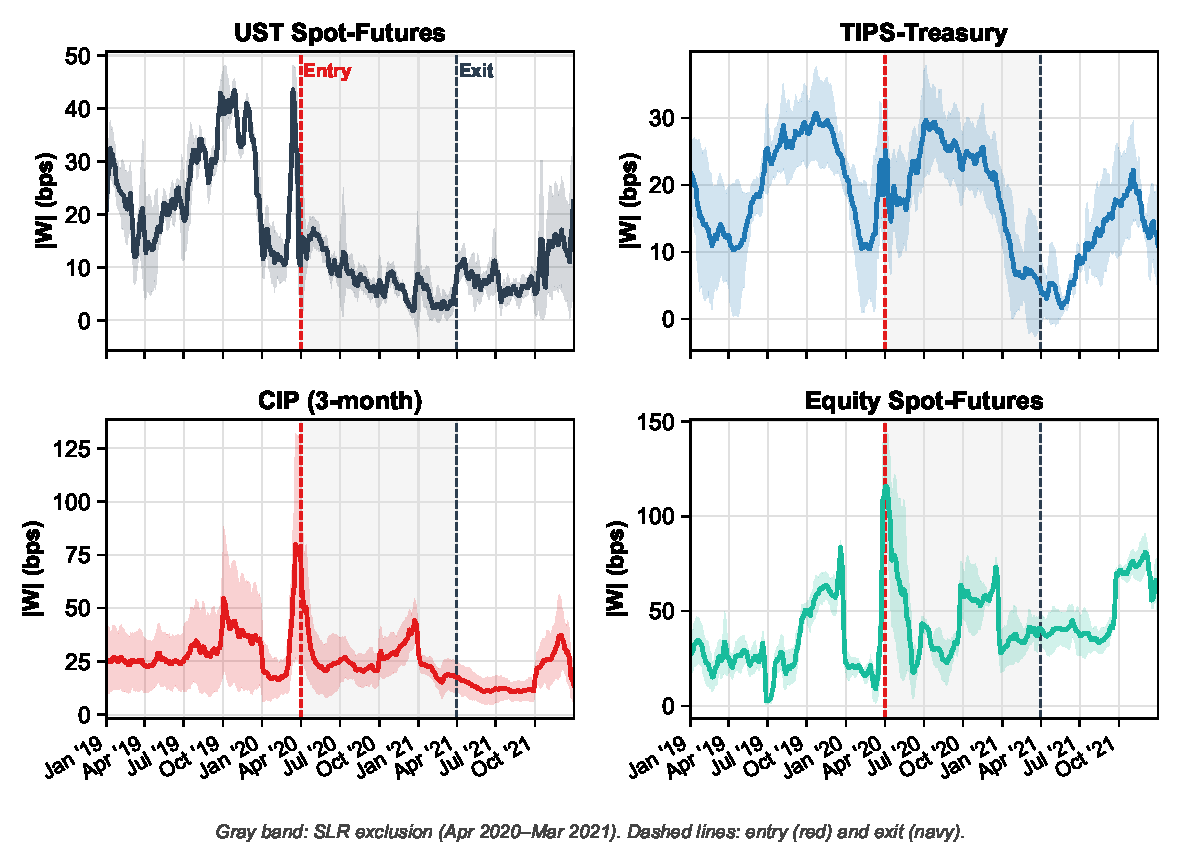
\includegraphics[width=0.95\textwidth]{figures_output/fig1_series_overview.pdf}
  \caption{Time-series evolution of arbitrage spreads, 2019--2021. Each panel shows the cross-series mean (solid line) and $\pm$1 standard deviation band (shaded) of absolute spread $|W|$ in basis points, smoothed with a 5-day rolling average. The gray shaded region denotes the SLR exclusion relief period (April 1, 2020 -- March 31, 2021). Dashed vertical lines mark the entry (red) and exit (green) dates.}
  \label{fig:series_overview}
\end{figure}

\begin{figure}[htbp]
  \centering
  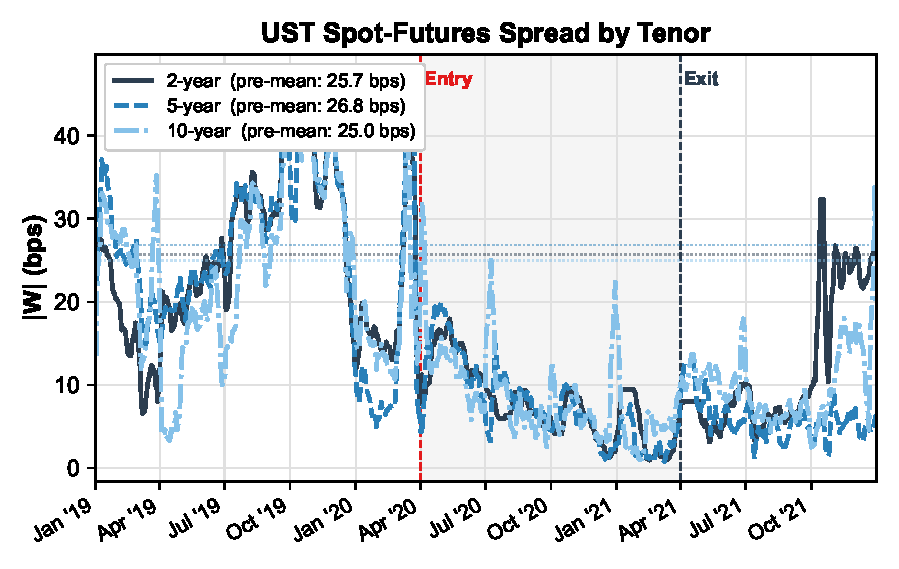
\includegraphics[width=0.95\textwidth]{figures_output/fig2_ust_sf_detail.pdf}
  \caption{UST spot-futures arbitrage spread by tenor, 2019--2021. Lines show the absolute spread $|W|$ for 2-year (solid), 5-year (dashed), and 10-year (dotted) maturities, smoothed with a 5-day rolling average. Horizontal dotted lines indicate the pre-period mean (January 2019 -- January 2020). }
  \label{fig:ust_sf_detail}
\end{figure}

\begin{figure}[htbp]
  \centering
  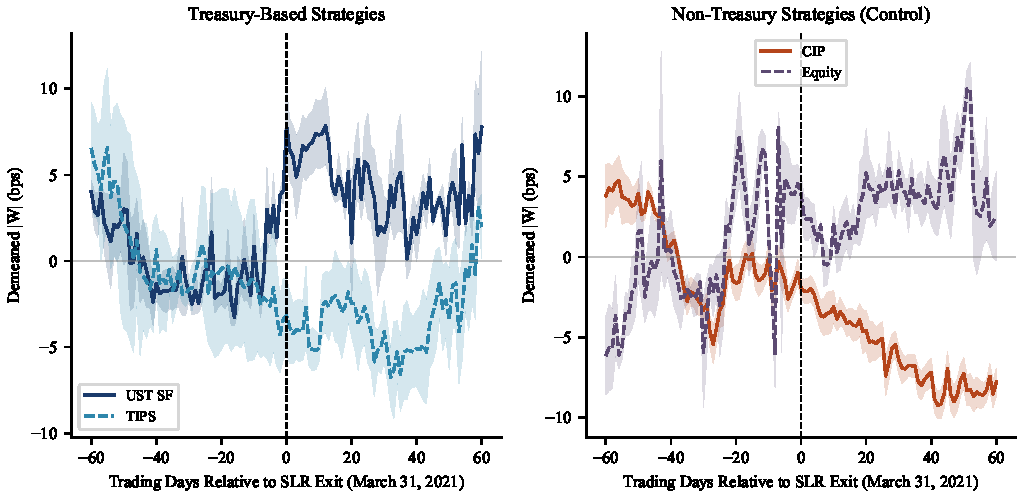
\includegraphics[width=0.95\textwidth]{figures_output/fig3_exit_event_paths.pdf}
  \caption{Event-time paths around the SLR exclusion exit (March 31, 2021). Left panel: Treasury-based strategies (UST spot-futures and TIPS-Treasury). Right panel: non-Treasury control strategies (CIP and Equity spot-futures). Series are demeaned by their pre-event mean (trading days $-60$ to $-1$) before averaging. Shaded bands denote $\pm$1 standard error. Dashed vertical line at day 0 marks the exit date.}
  \label{fig:exit_event_paths}
\end{figure}

\begin{figure}[htbp]
  \centering
  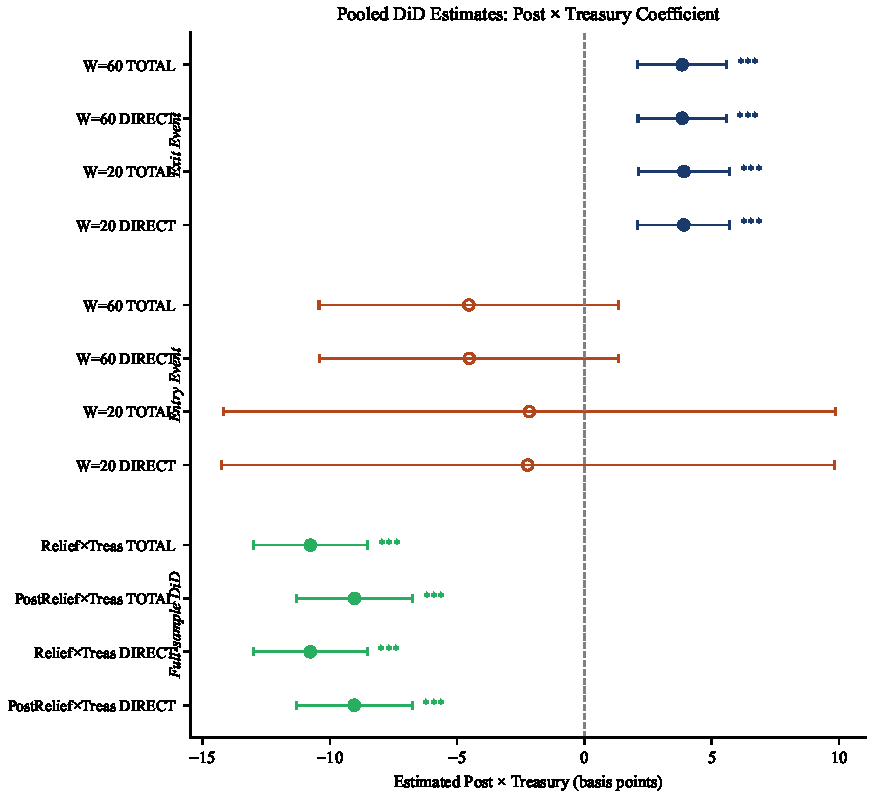
\includegraphics[width=0.95\textwidth]{figures_output/fig4_coef_plot.pdf}
  \caption{Pooled difference-in-differences estimates of the Post$\times$Treasury coefficient. Each row reports a point estimate with 95\% confidence interval. Exit and Entry event estimates use windows $W\in\{20,60\}$ trading days; Full-sample DiD estimates span 2019--2021. Filled markers indicate $|t|>1.645$; stars denote $|t|>1.96$ (**) and $|t|>2.576$ (***).}
  \label{fig:coef_plot}
\end{figure}

\begin{figure}[htbp]
  \centering
  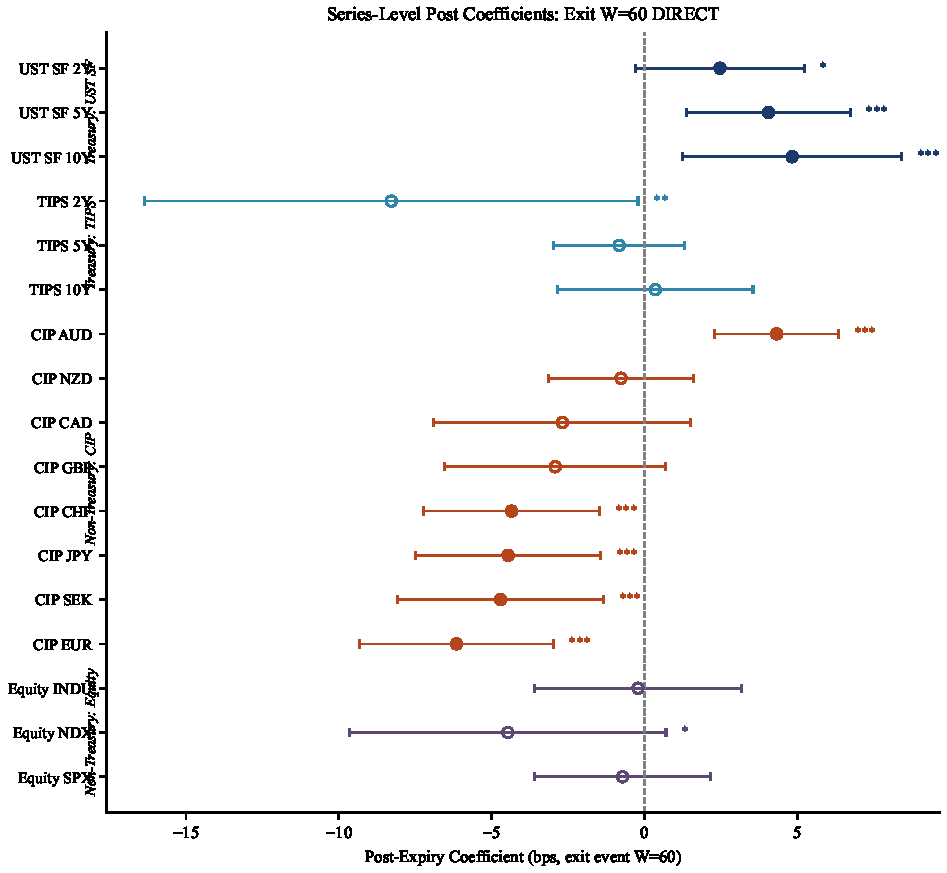
\includegraphics[width=0.95\textwidth]{figures_output/fig5_series_level_coefs.pdf}
  \caption{Series-level post-expiry coefficients for the exit event (March 31, 2021), window $W=60$, DIRECT specification. Each row is an individual series; error bars show 95\% confidence intervals. Filled markers indicate $|t|>1.645$.}
  \label{fig:series_level_coefs}
\end{figure}

\begin{figure}[htbp]
  \centering
  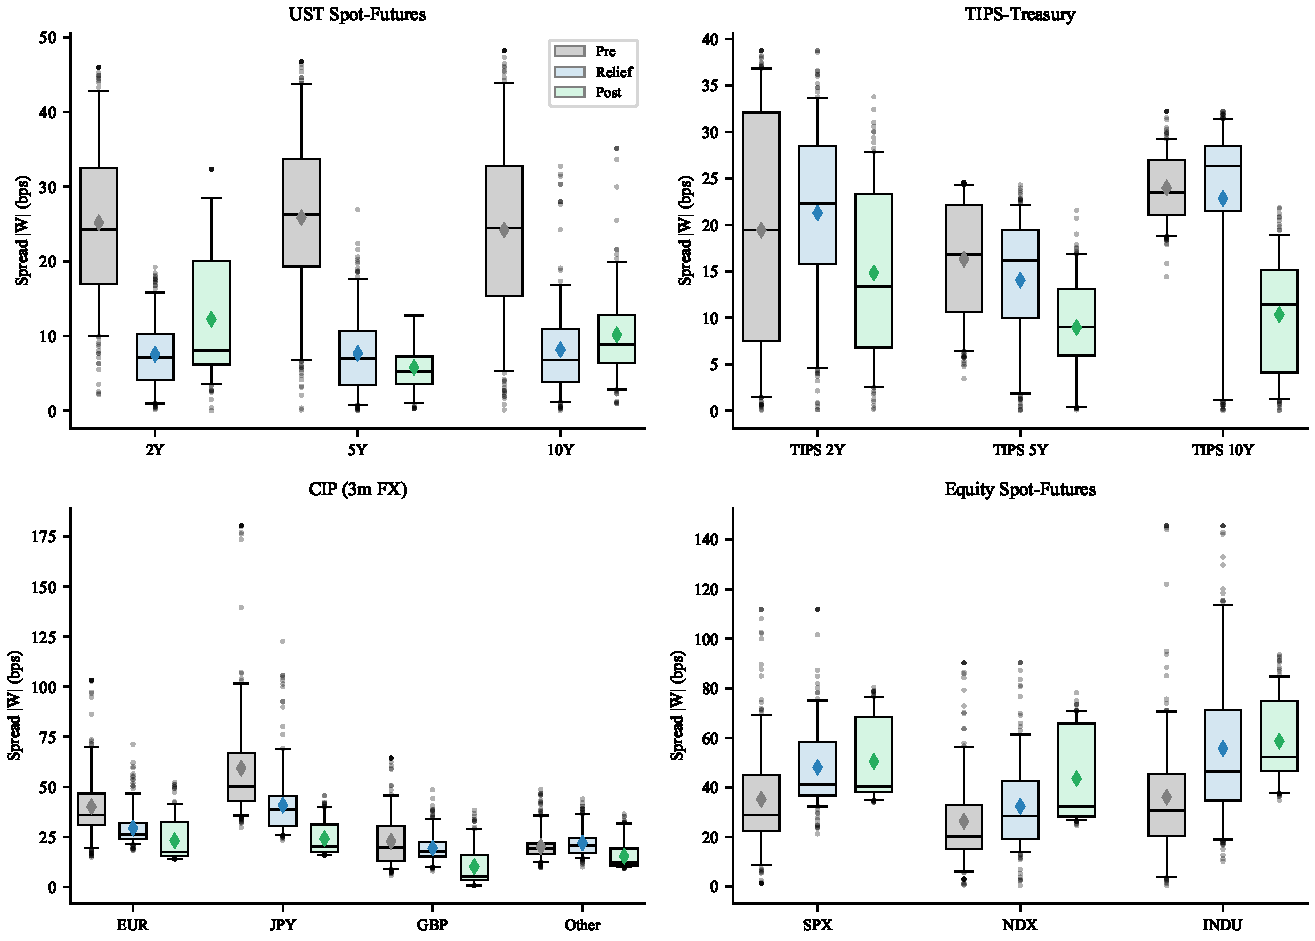
\includegraphics[width=0.95\textwidth]{figures_output/fig6_regime_boxplots.pdf}
  \caption{Distribution of absolute arbitrage spreads $|W|$ by regime and strategy. Box spans the interquartile range; whiskers extend to the 5th and 95th percentiles; diamonds mark the within-group mean. Pre = January 2019 -- March 31, 2020; Relief = April 1, 2020 -- March 31, 2021; Post = April 1 -- December 31, 2021.}
  \label{fig:regime_boxplots}
\end{figure}

 in your main .tex file

\begin{figure}[htbp]
  \centering
  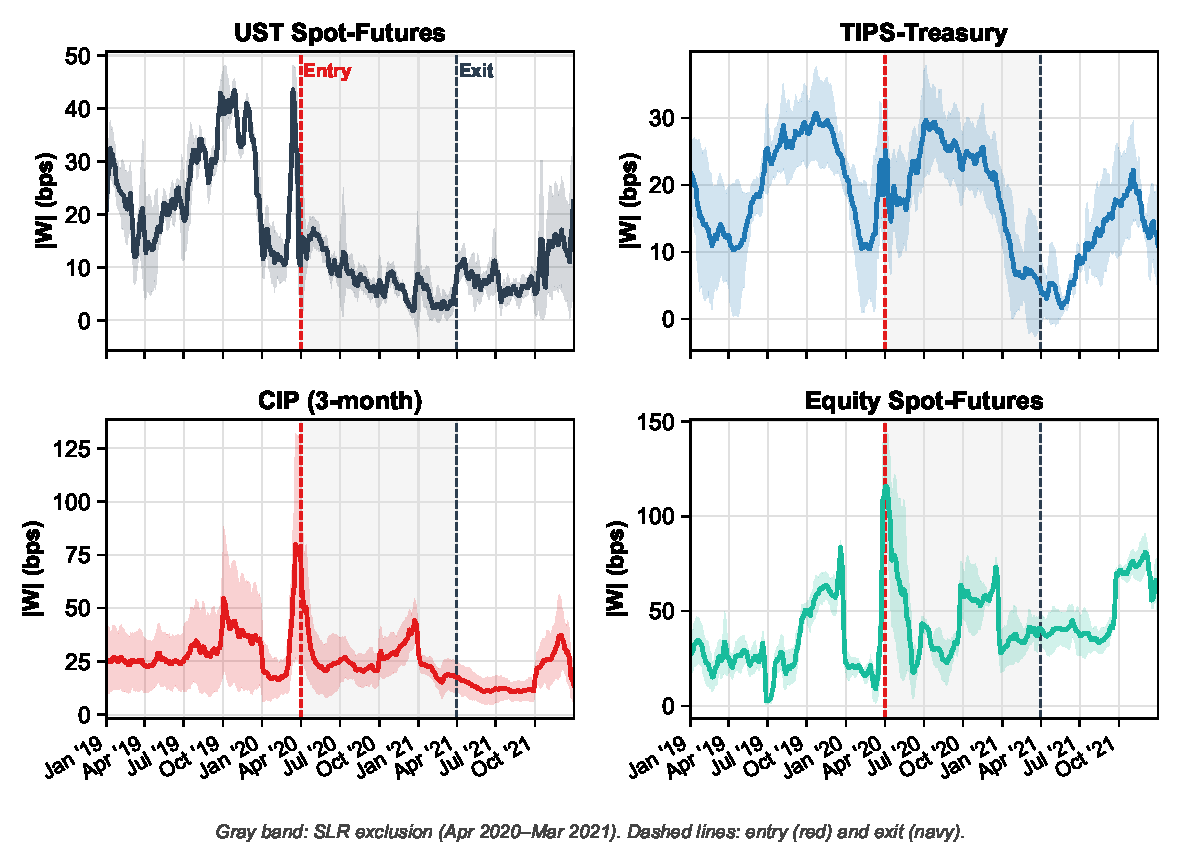
\includegraphics[width=0.95\textwidth]{figures_output/fig1_series_overview.pdf}
  \caption{Time-series evolution of arbitrage spreads, 2019--2021. Each panel shows the cross-series mean (solid line) and $\pm$1 standard deviation band (shaded) of absolute spread $|W|$ in basis points, smoothed with a 5-day rolling average. The gray shaded region denotes the SLR exclusion relief period (April 1, 2020 -- March 31, 2021). Dashed vertical lines mark the entry (red) and exit (green) dates.}
  \label{fig:series_overview}
\end{figure}

\begin{figure}[htbp]
  \centering
  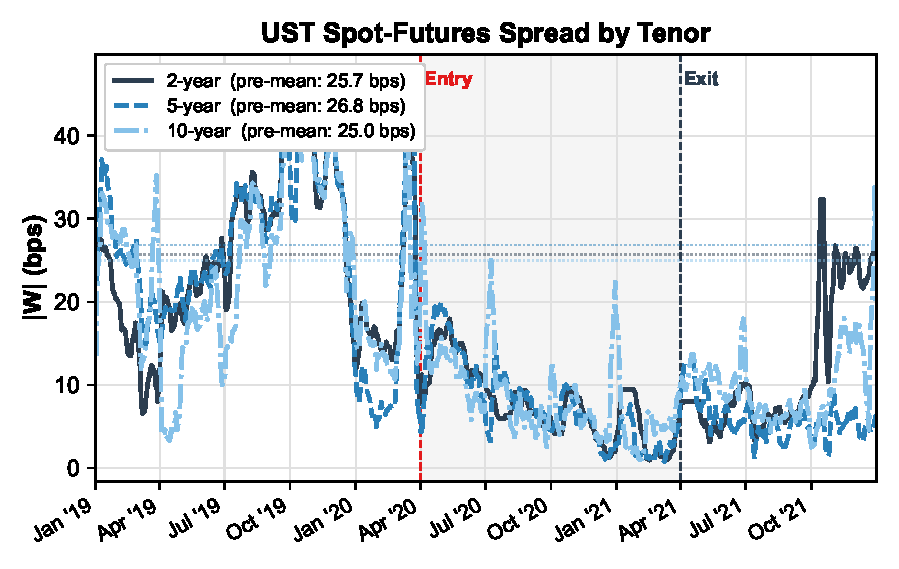
\includegraphics[width=0.95\textwidth]{figures_output/fig2_ust_sf_detail.pdf}
  \caption{UST spot-futures arbitrage spread by tenor, 2019--2021. Lines show the absolute spread $|W|$ for 2-year (solid), 5-year (dashed), and 10-year (dotted) maturities, smoothed with a 5-day rolling average. Horizontal dotted lines indicate the pre-period mean (January 2019 -- January 2020). }
  \label{fig:ust_sf_detail}
\end{figure}

\begin{figure}[htbp]
  \centering
  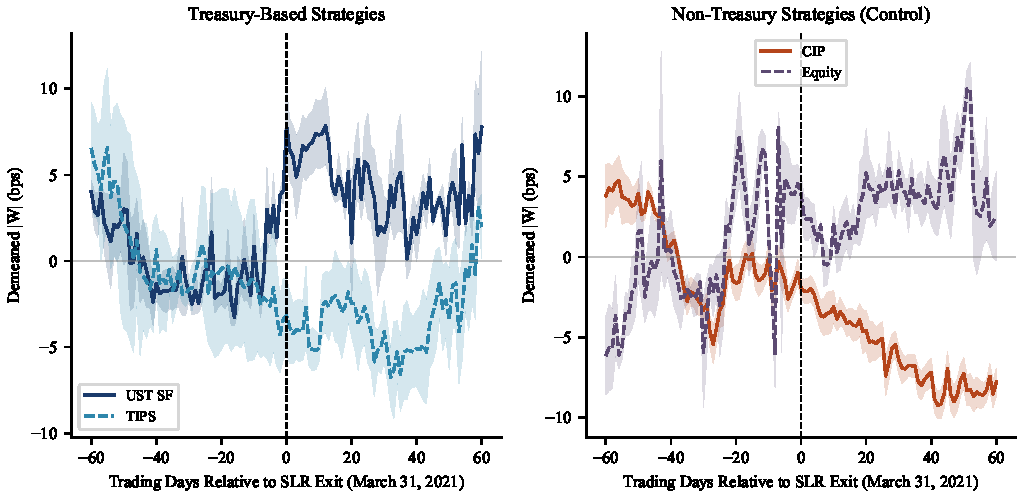
\includegraphics[width=0.95\textwidth]{figures_output/fig3_exit_event_paths.pdf}
  \caption{Event-time paths around the SLR exclusion exit (March 31, 2021). Left panel: Treasury-based strategies (UST spot-futures and TIPS-Treasury). Right panel: non-Treasury control strategies (CIP and Equity spot-futures). Series are demeaned by their pre-event mean (trading days $-60$ to $-1$) before averaging. Shaded bands denote $\pm$1 standard error. Dashed vertical line at day 0 marks the exit date.}
  \label{fig:exit_event_paths}
\end{figure}

\begin{figure}[htbp]
  \centering
  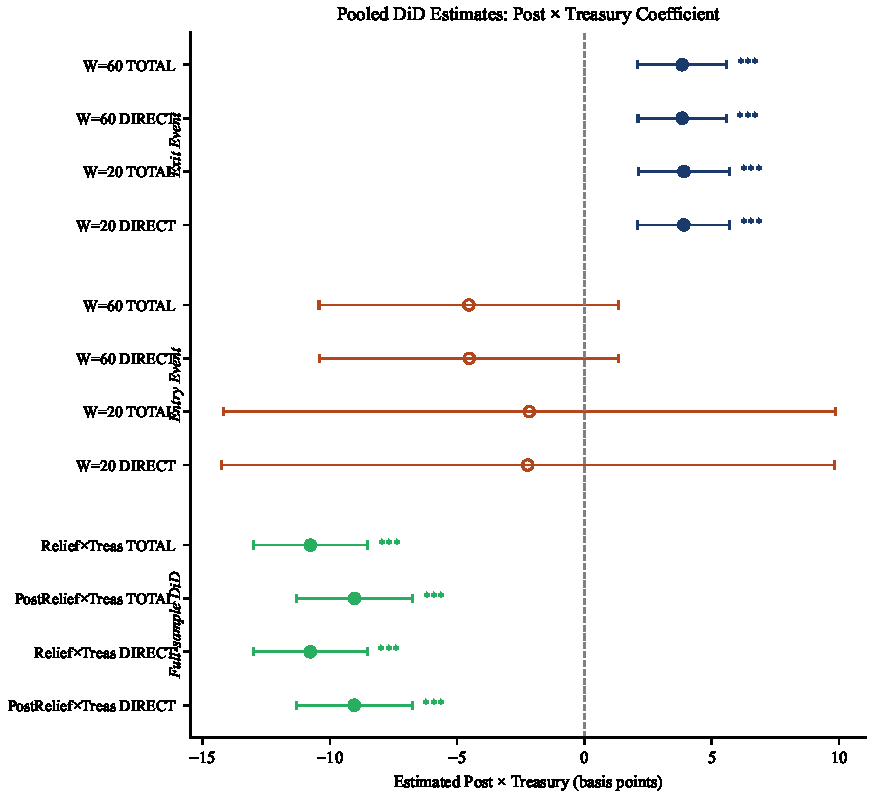
\includegraphics[width=0.95\textwidth]{figures_output/fig4_coef_plot.pdf}
  \caption{Pooled difference-in-differences estimates of the Post$\times$Treasury coefficient. Each row reports a point estimate with 95\% confidence interval. Exit and Entry event estimates use windows $W\in\{20,60\}$ trading days; Full-sample DiD estimates span 2019--2021. Filled markers indicate $|t|>1.645$; stars denote $|t|>1.96$ (**) and $|t|>2.576$ (***).}
  \label{fig:coef_plot}
\end{figure}

\begin{figure}[htbp]
  \centering
  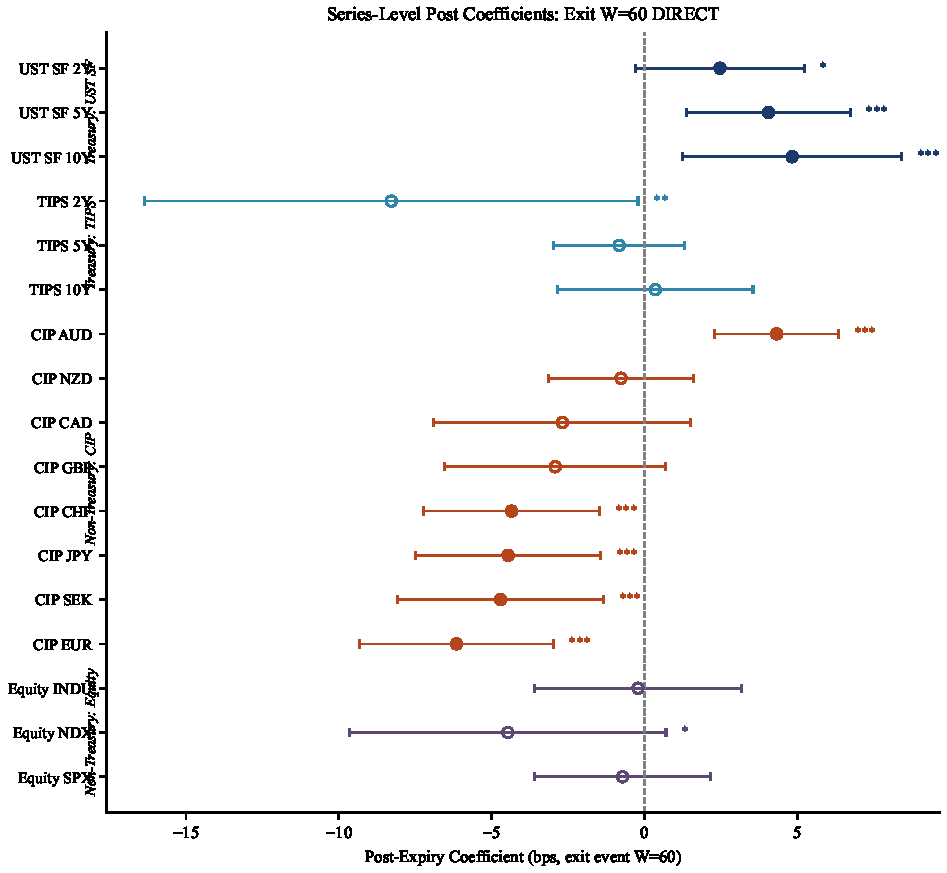
\includegraphics[width=0.95\textwidth]{figures_output/fig5_series_level_coefs.pdf}
  \caption{Series-level post-expiry coefficients for the exit event (March 31, 2021), window $W=60$, DIRECT specification. Each row is an individual series; error bars show 95\% confidence intervals. Filled markers indicate $|t|>1.645$.}
  \label{fig:series_level_coefs}
\end{figure}

\begin{figure}[htbp]
  \centering
  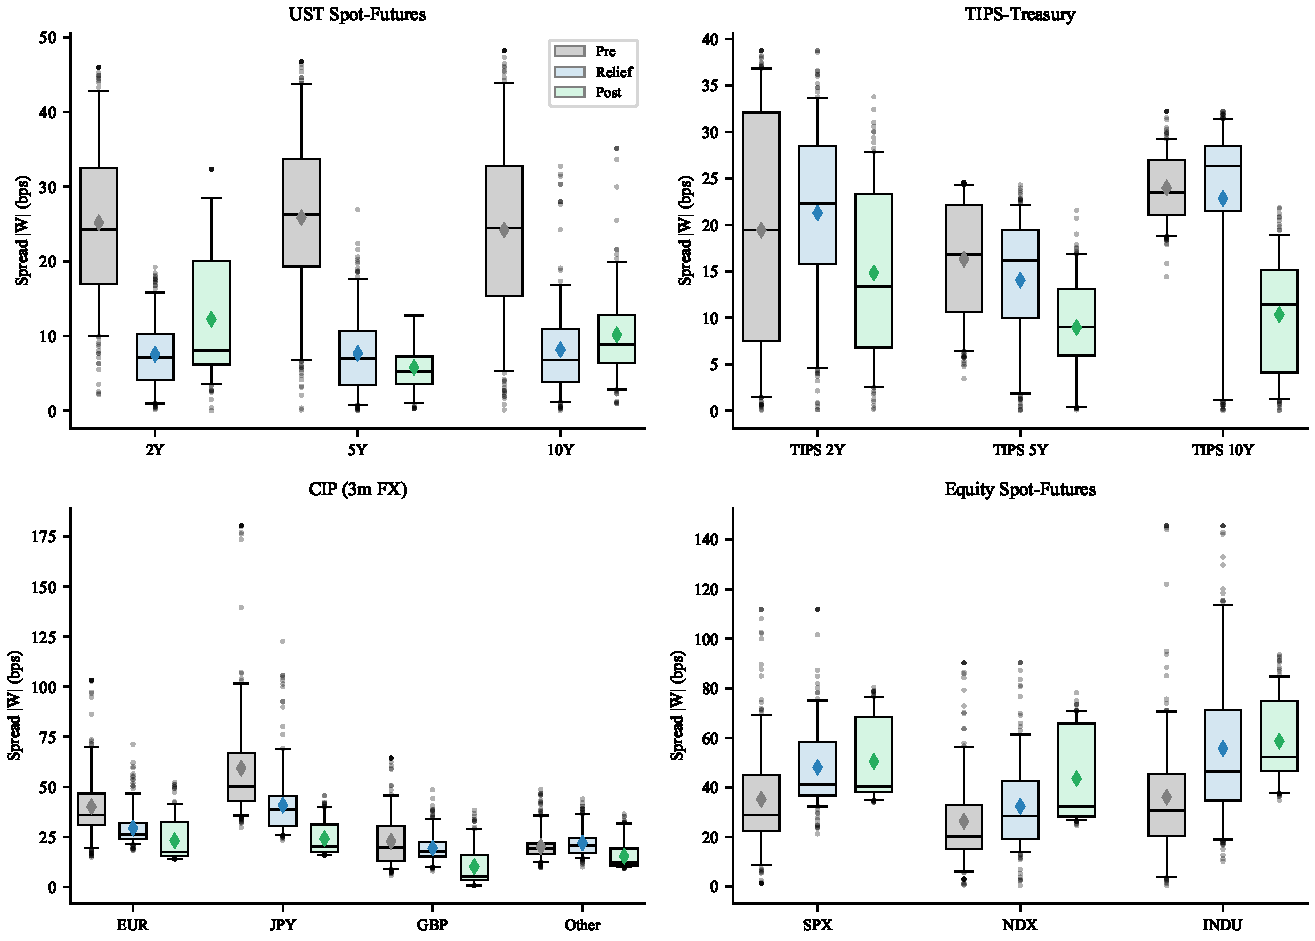
\includegraphics[width=0.95\textwidth]{figures_output/fig6_regime_boxplots.pdf}
  \caption{Distribution of absolute arbitrage spreads $|W|$ by regime and strategy. Box spans the interquartile range; whiskers extend to the 5th and 95th percentiles; diamonds mark the within-group mean. Pre = January 2019 -- March 31, 2020; Relief = April 1, 2020 -- March 31, 2021; Post = April 1 -- December 31, 2021.}
  \label{fig:regime_boxplots}
\end{figure}

 in your main .tex file

\begin{figure}[htbp]
  \centering
  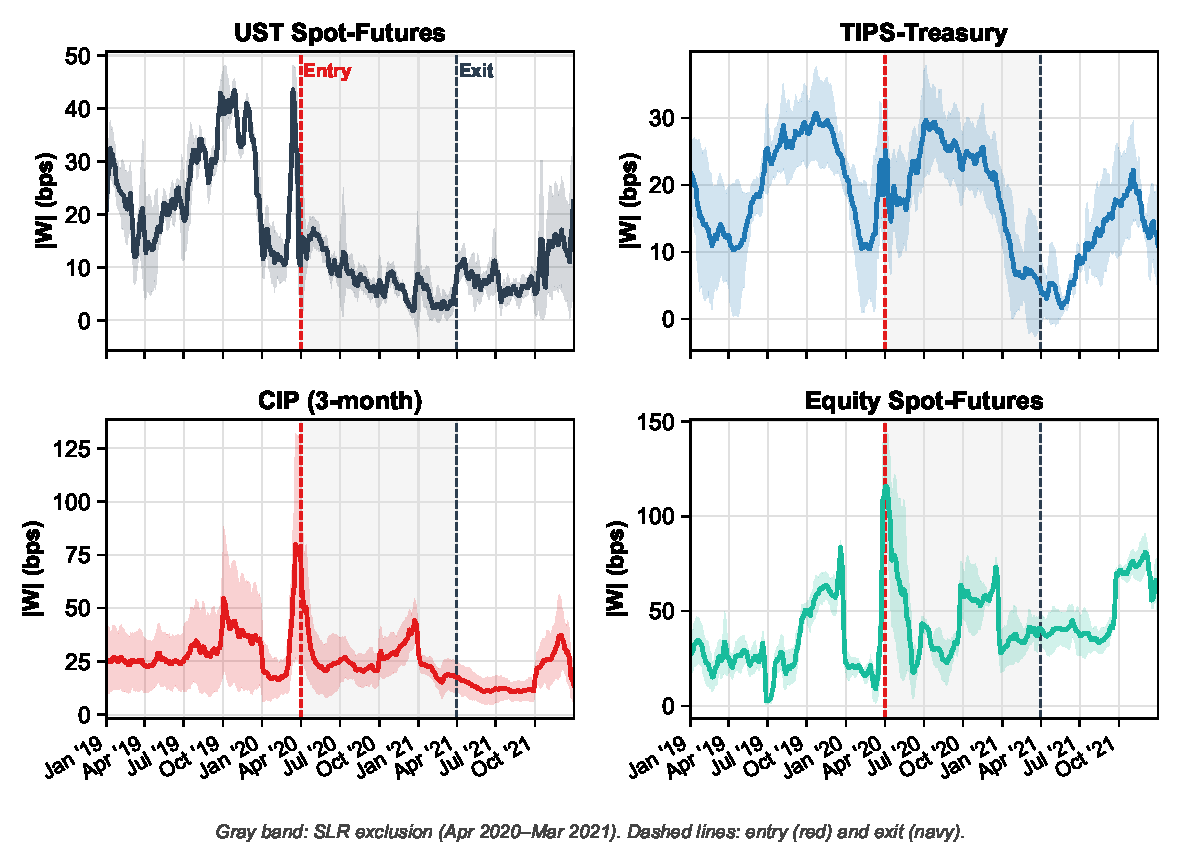
\includegraphics[width=0.95\textwidth]{figures_output/fig1_series_overview.pdf}
  \caption{Time-series evolution of arbitrage spreads, 2019--2021. Each panel shows the cross-series mean (solid line) and $\pm$1 standard deviation band (shaded) of absolute spread $|W|$ in basis points, smoothed with a 5-day rolling average. The gray shaded region denotes the SLR exclusion relief period (April 1, 2020 -- March 31, 2021). Dashed vertical lines mark the entry (red) and exit (green) dates.}
  \label{fig:series_overview}
\end{figure}

\begin{figure}[htbp]
  \centering
  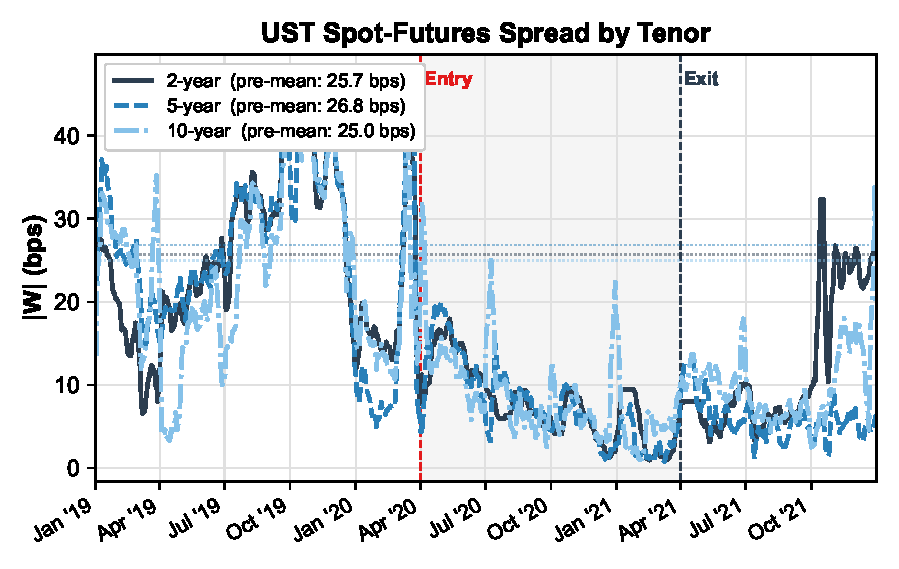
\includegraphics[width=0.95\textwidth]{figures_output/fig2_ust_sf_detail.pdf}
  \caption{UST spot-futures arbitrage spread by tenor, 2019--2021. Lines show the absolute spread $|W|$ for 2-year (solid), 5-year (dashed), and 10-year (dotted) maturities, smoothed with a 5-day rolling average. Horizontal dotted lines indicate the pre-period mean (January 2019 -- January 2020). }
  \label{fig:ust_sf_detail}
\end{figure}

\begin{figure}[htbp]
  \centering
  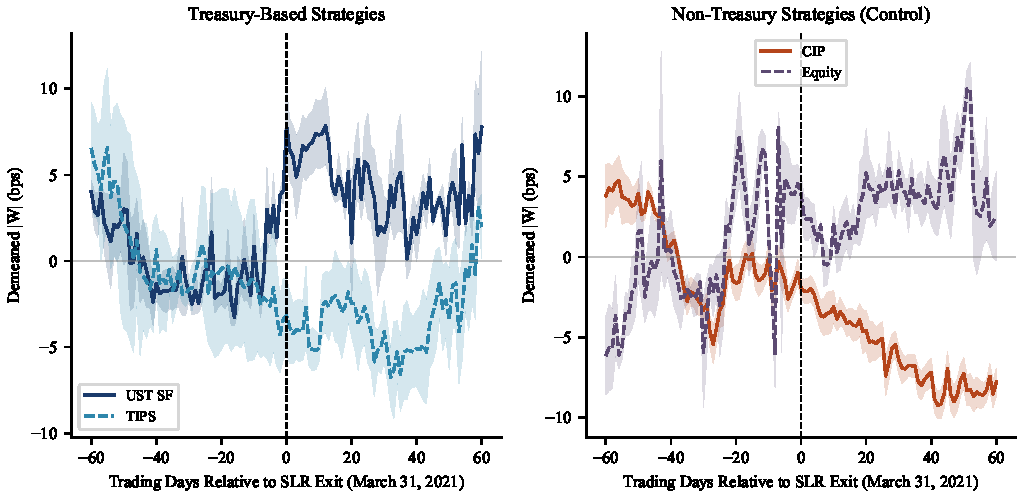
\includegraphics[width=0.95\textwidth]{figures_output/fig3_exit_event_paths.pdf}
  \caption{Event-time paths around the SLR exclusion exit (March 31, 2021). Left panel: Treasury-based strategies (UST spot-futures and TIPS-Treasury). Right panel: non-Treasury control strategies (CIP and Equity spot-futures). Series are demeaned by their pre-event mean (trading days $-60$ to $-1$) before averaging. Shaded bands denote $\pm$1 standard error. Dashed vertical line at day 0 marks the exit date.}
  \label{fig:exit_event_paths}
\end{figure}

\begin{figure}[htbp]
  \centering
  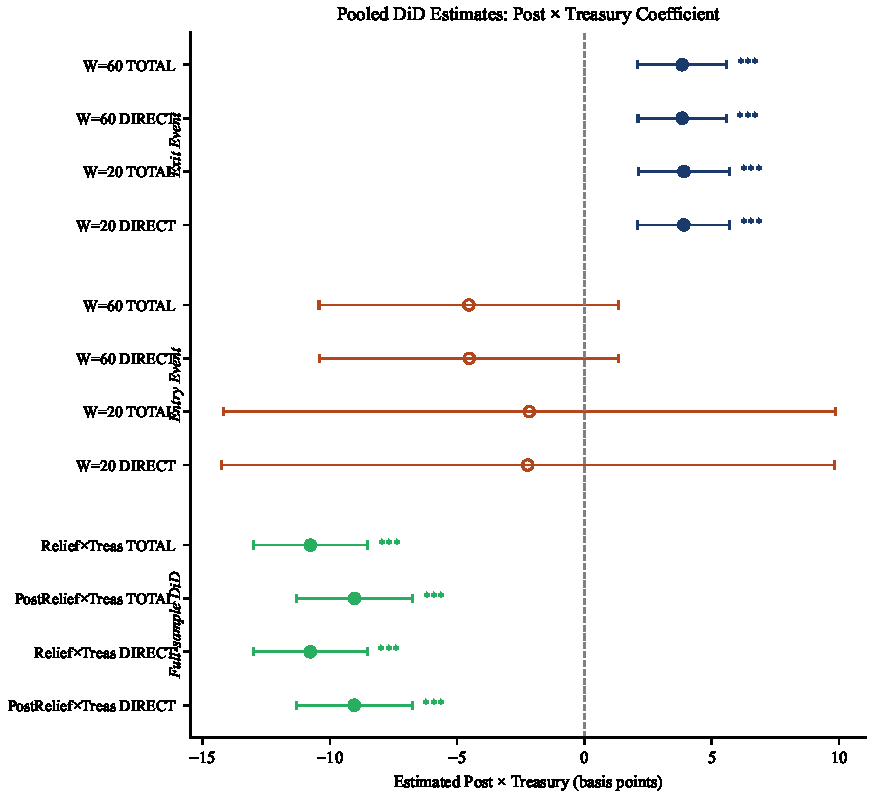
\includegraphics[width=0.95\textwidth]{figures_output/fig4_coef_plot.pdf}
  \caption{Pooled difference-in-differences estimates of the Post$\times$Treasury coefficient. Each row reports a point estimate with 95\% confidence interval. Exit and Entry event estimates use windows $W\in\{20,60\}$ trading days; Full-sample DiD estimates span 2019--2021. Filled markers indicate $|t|>1.645$; stars denote $|t|>1.96$ (**) and $|t|>2.576$ (***).}
  \label{fig:coef_plot}
\end{figure}

\begin{figure}[htbp]
  \centering
  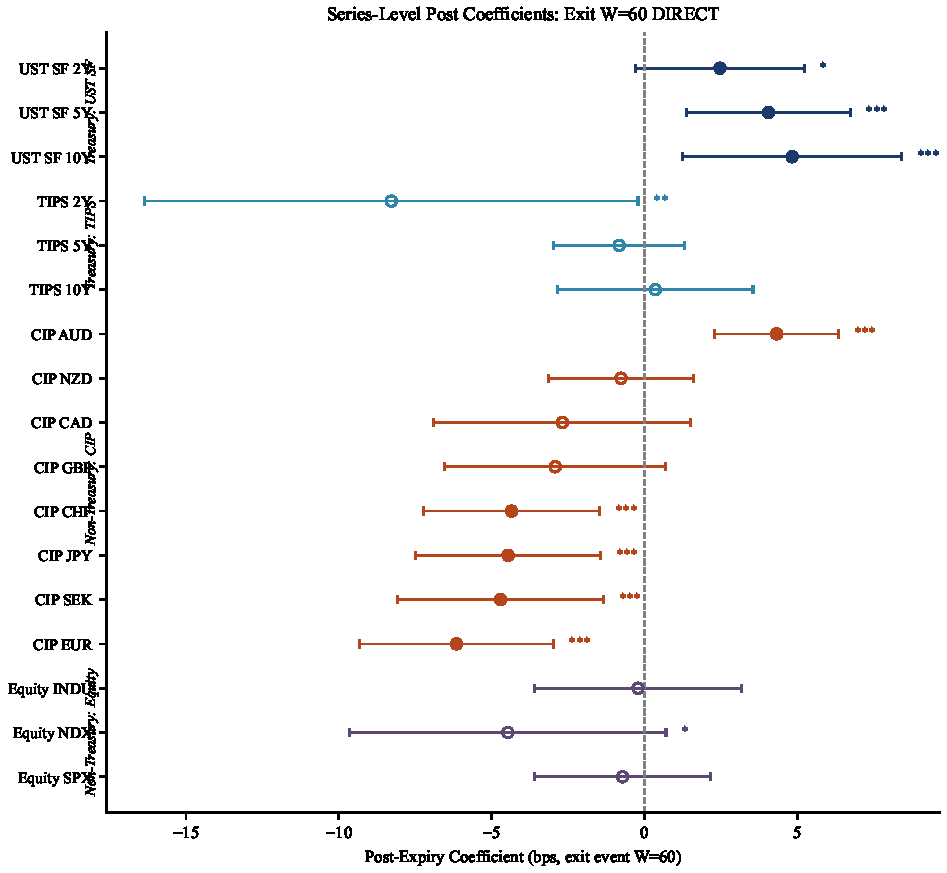
\includegraphics[width=0.95\textwidth]{figures_output/fig5_series_level_coefs.pdf}
  \caption{Series-level post-expiry coefficients for the exit event (March 31, 2021), window $W=60$, DIRECT specification. Each row is an individual series; error bars show 95\% confidence intervals. Filled markers indicate $|t|>1.645$.}
  \label{fig:series_level_coefs}
\end{figure}

\begin{figure}[htbp]
  \centering
  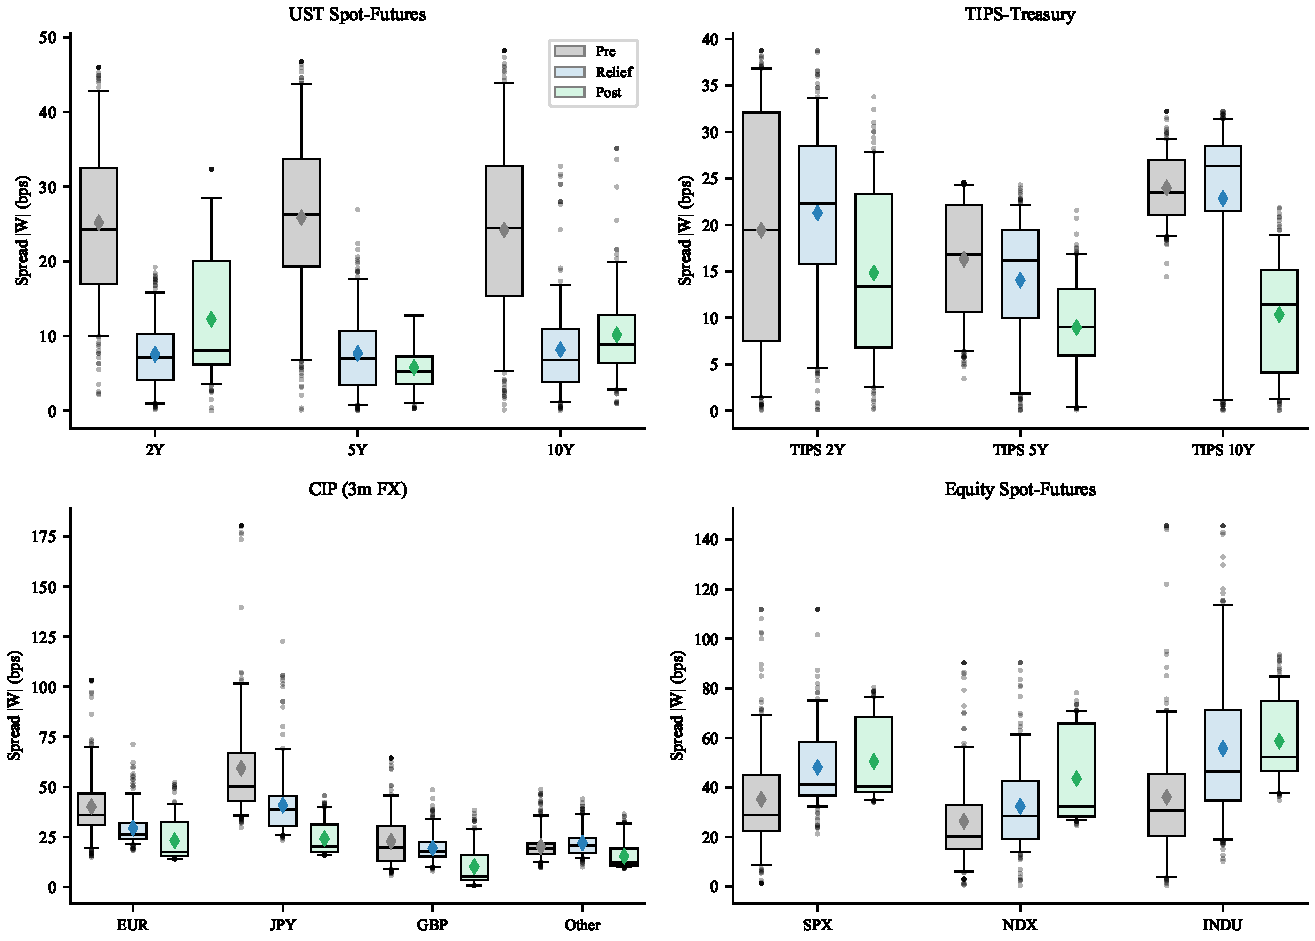
\includegraphics[width=0.95\textwidth]{figures_output/fig6_regime_boxplots.pdf}
  \caption{Distribution of absolute arbitrage spreads $|W|$ by regime and strategy. Box spans the interquartile range; whiskers extend to the 5th and 95th percentiles; diamonds mark the within-group mean. Pre = January 2019 -- March 31, 2020; Relief = April 1, 2020 -- March 31, 2021; Post = April 1 -- December 31, 2021.}
  \label{fig:regime_boxplots}
\end{figure}

 in your main .tex file

\begin{figure}[htbp]
  \centering
  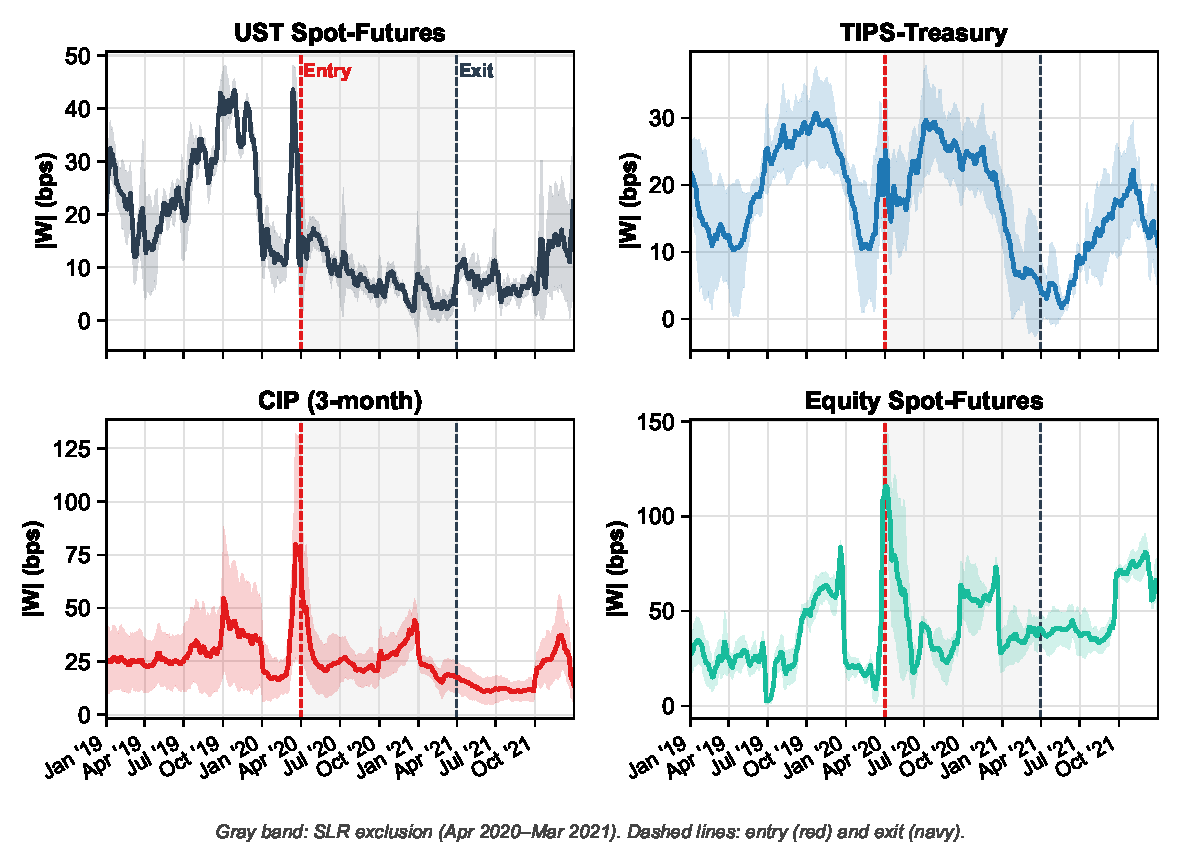
\includegraphics[width=0.95\textwidth]{figures_output/fig1_series_overview.pdf}
  \caption{Time-series evolution of arbitrage spreads, 2019--2021. Each panel shows the cross-series mean (solid line) and $\pm$1 standard deviation band (shaded) of absolute spread $|W|$ in basis points, smoothed with a 5-day rolling average. The gray shaded region denotes the SLR exclusion relief period (April~1, 2020 -- March~31, 2021). Dashed vertical lines mark the entry (red) and exit (green) dates.}
  \label{fig:series_overview}
\end{figure}

\begin{figure}[htbp]
  \centering
  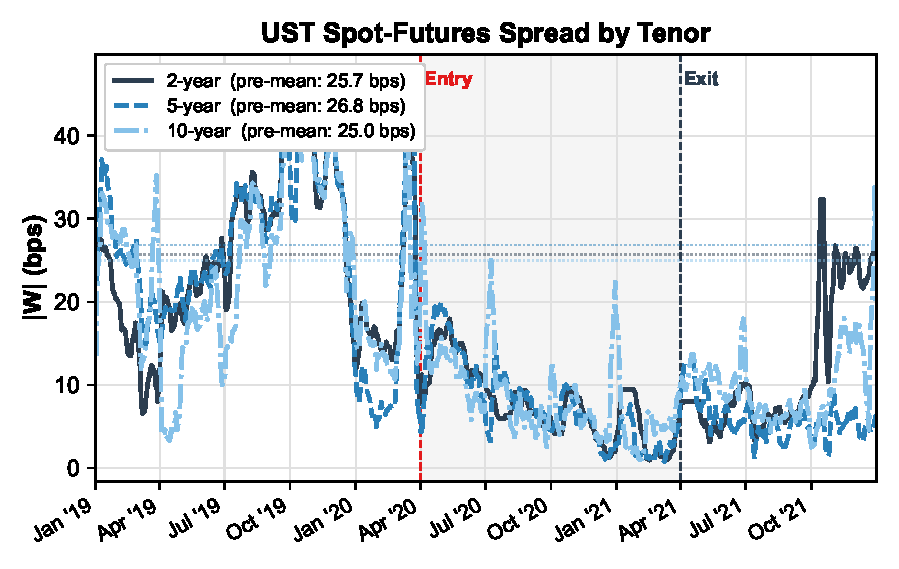
\includegraphics[width=0.95\textwidth]{figures_output/fig2_ust_sf_detail.pdf}
  \caption{UST spot-futures arbitrage spread by tenor, 2019--2021. Lines show the absolute spread $|W|$ for 2-year (solid), 5-year (dashed), and 10-year (dotted) maturities, smoothed with a 5-day rolling average. Dotted horizontal lines indicate the pre-period mean (January~2019 -- January~2020); values are reported in the legend. }
  \label{fig:ust_sf_detail}
\end{figure}

\begin{figure}[htbp]
  \centering
  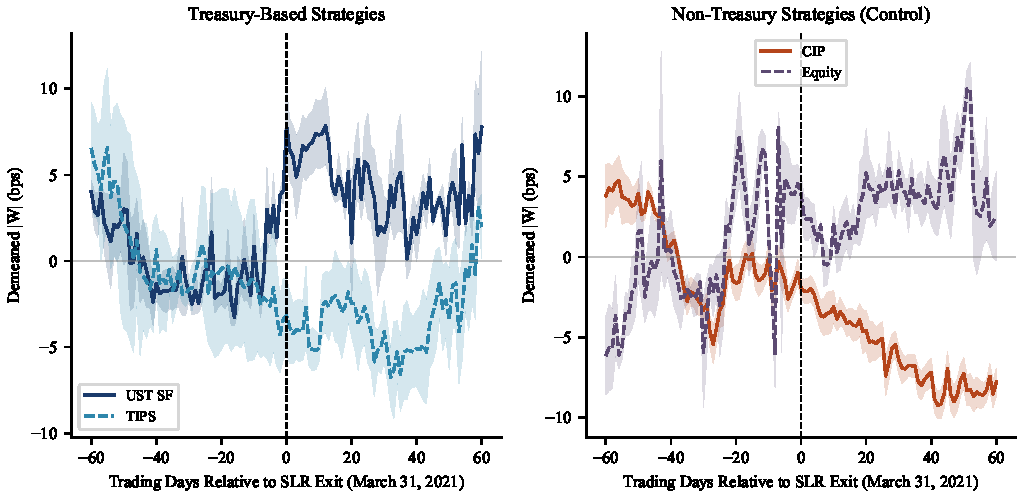
\includegraphics[width=0.95\textwidth]{figures_output/fig3_exit_event_paths.pdf}
  \caption{Event-time paths around the SLR exclusion exit (March~31, 2021). Left panel: Treasury-based strategies (UST spot-futures and TIPS-Treasury). Right panel: non-Treasury control strategies (CIP and equity spot-futures). Series are demeaned by their pre-event mean (trading days $-60$ to $-1$) before averaging. Shaded bands denote $\pm$1 standard error. Dashed vertical line at day 0 marks the exit date.}
  \label{fig:exit_event_paths}
\end{figure}

\begin{figure}[htbp]
  \centering
  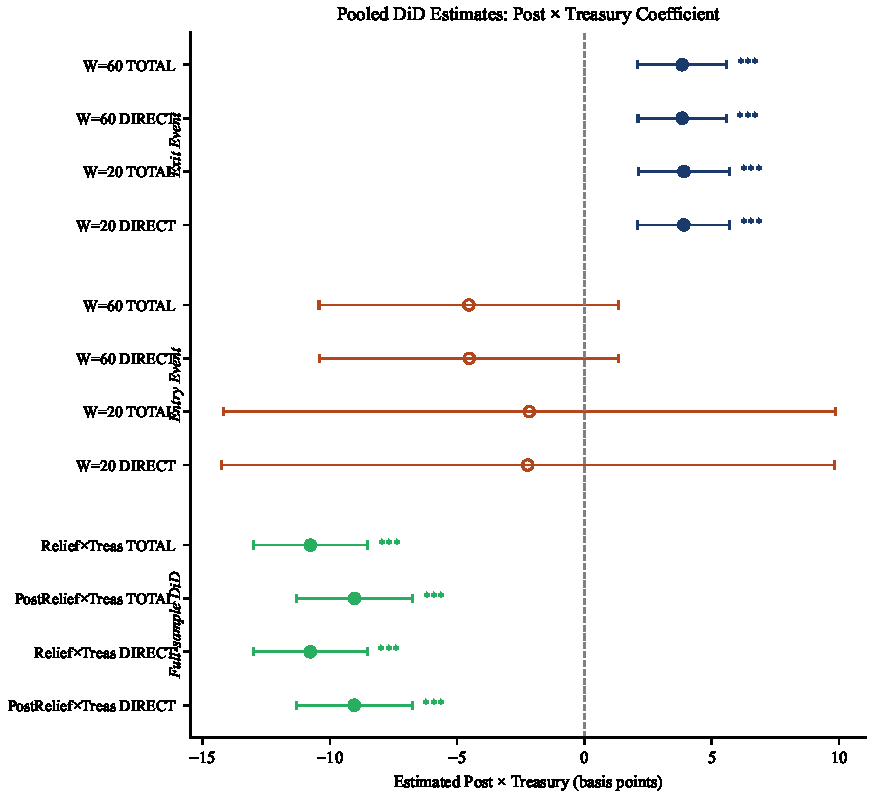
\includegraphics[width=0.95\textwidth]{figures_output/fig4_coef_plot.pdf}
  \caption{Pooled difference-in-differences estimates of the Post$\times$Treasury coefficient. Each row reports a point estimate with 95\% confidence interval (HAC, Newey-West 5 lags). Exit and entry event estimates use windows $W\in\{20,60\}$ trading days; full-period DiD estimates span 2019--2021 with 2019 as the clean pre-COVID baseline. Filled markers: $|t|>1.645$; stars: $|t|>1.96$ (**) and $|t|>2.576$ (***).}
  \label{fig:coef_plot}
\end{figure}

\begin{figure}[htbp]
  \centering
  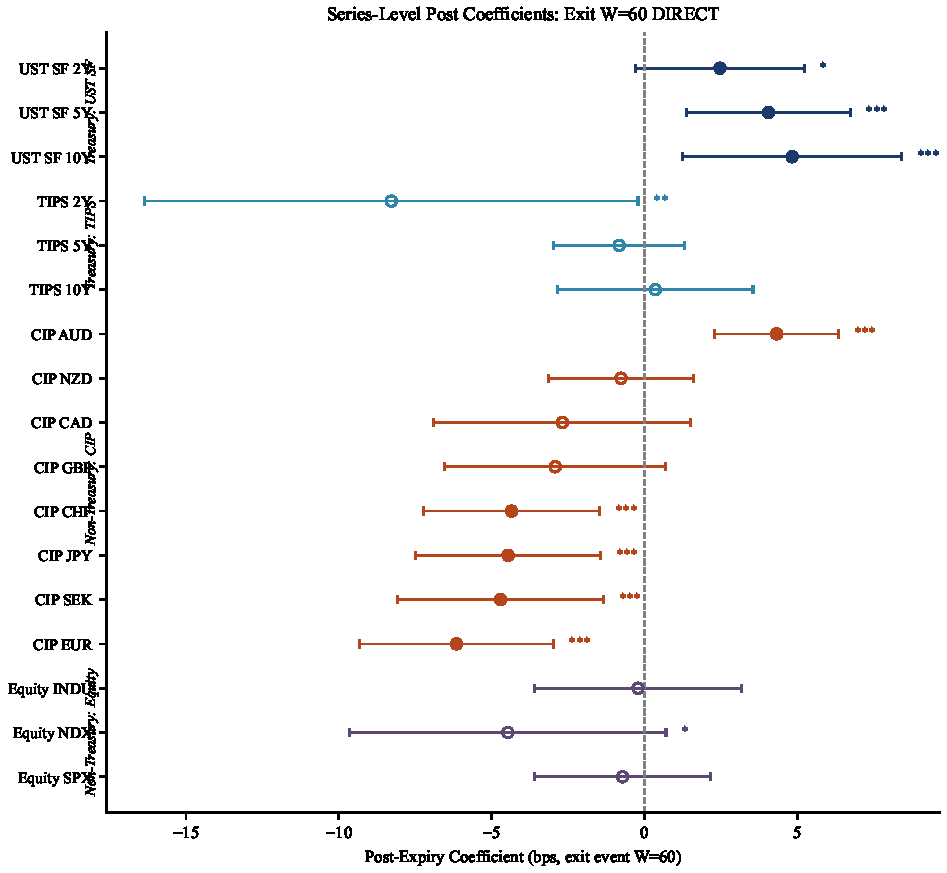
\includegraphics[width=0.95\textwidth]{figures_output/fig5_series_level_coefs.pdf}
  \caption{Series-level post-expiry coefficients for the exit event (March~31, 2021), window $W=60$, \textsc{Direct} specification. Each row is an individual series; error bars show 95\% confidence intervals (HAC). Filled markers: $|t|>1.645$. Group headers in bold italic; separator lines between strategy classes.}
  \label{fig:series_level_coefs}
\end{figure}

\begin{figure}[htbp]
  \centering
  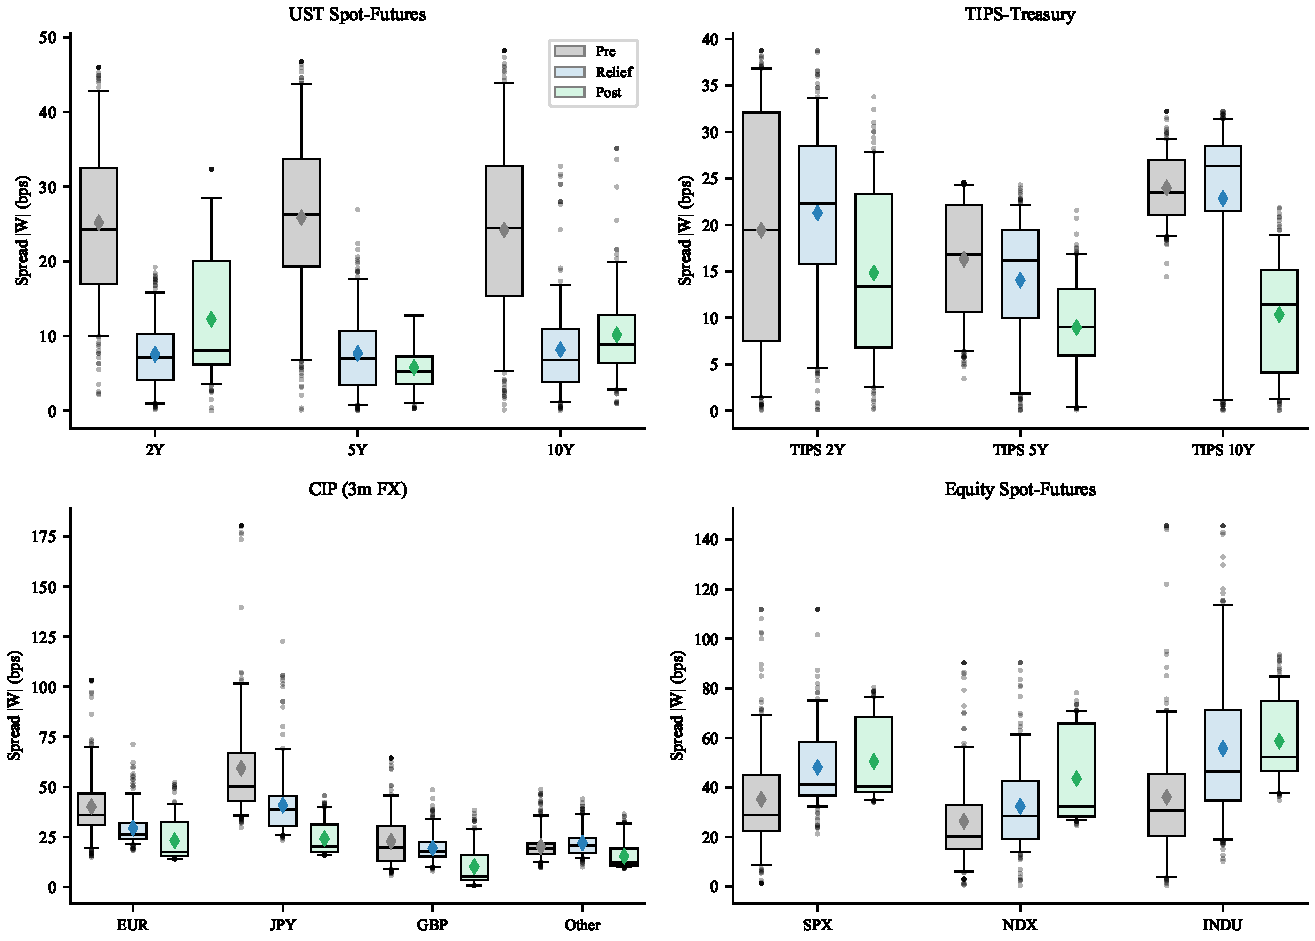
\includegraphics[width=0.95\textwidth]{figures_output/fig6_regime_boxplots.pdf}
  \caption{Distribution of absolute arbitrage spreads $|W|$ by regime and strategy. Boxes span the interquartile range; whiskers extend to the 5th and 95th percentiles; diamonds mark the within-group mean. Pre = January~2019 -- March~31, 2020; Relief = April~1, 2020 -- March~31, 2021; Post = April~1 -- December~31, 2021.}
  \label{fig:regime_boxplots}
\end{figure}

